%%%%%%%%%%%%%%%%%%%%%%%%%%%%%%%%%%%%%%%%%
% Structured General Purpose Assignment
% LaTeX Template
%
% This template has been downloaded from:
% http://www.latextemplates.com
%
% Original author:
% Ted Pavlic (http://www.tedpavlic.com)
%
% Note:
% The \lipsum[#] commands throughout this template generate dummy text
% to fill the template out. These commands should all be removed when 
% writing assignment content.
%
%%%%%%%%%%%%%%%%%%%%%%%%%%%%%%%%%%%%%%%%%

\documentclass{article}

\usepackage{fancyhdr} % Required for custom headers
\usepackage{lastpage} % Required to determine the last page for the footer
\usepackage{extramarks} % Required for headers and footers
\usepackage{graphicx} % Required to insert images
\usepackage[latin1]{inputenc}

% Margins
\topmargin=-0.45in
\evensidemargin=0in
\oddsidemargin=0in
\textwidth=6.5in
\textheight=9.0in
\headsep=0.25in 

\linespread{1.1} % Line spacing



\setlength\parindent{0pt} % Removes all indentation from paragraphs

%----------------------------------------------------------------------------------------
%	DOCUMENT STRUCTURE COMMANDS
%	Skip this unless you know what you're doing
%----------------------------------------------------------------------------------------

% Header and footer for when a page split occurs within a problem environment
\newcommand{\enterProblemHeader}[1]{
\nobreak\extramarks{#1}{#1 continued on next page\ldots}\nobreak
\nobreak\extramarks{#1 (continued)}{#1 continued on next page\ldots}\nobreak
}

% Header and footer for when a page split occurs between problem environments
\newcommand{\exitProblemHeader}[1]{
\nobreak\extramarks{#1 (continued)}{#1 continued on next page\ldots}\nobreak
\nobreak\extramarks{#1}{}\nobreak
}

\setcounter{secnumdepth}{0} % Removes default section numbers
\newcounter{homeworkProblemCounter} % Creates a counter to keep track of the number of problems
%----------------------------------------------------------------------------------------
%	NAME AND CLASS SECTION
%----------------------------------------------------------------------------------------

\newcommand{\lessonNumber}[1]{Lezione\ \##1} % Assignment title
\newcommand{\lessonDate}[4]{#1,\ #2\ #3\ #4} % Due date
\newcommand{\lessonCourse}[1]{#1} % Course/class
\newcommand{\lessonTime}[1]{#1} % Class/lecture time
\newcommand{\lessonTeacher}[1]{#1} % Teacher/lecturer
\newcommand{\lessonAuthor}[1]{#1} % Your name

% Set up the header and footer
\pagestyle{fancy}
\lhead{\lessonAuthor{Luca De Franceschi}} % Top left header
\chead{\lessonAuthor{Tullio Vardanega}\ \lessonTime{09:30}: \lessonNumber{21}} % Top center header
\rhead{\firstxmark} % Top right header
\lfoot{\lastxmark} % Bottom left footer
\cfoot{} % Bottom center footer
\rfoot{Page\ \thepage\ of\ \pageref{LastPage}} % Bottom right footer
\renewcommand\headrulewidth{0.4pt} % Size of the header rule
\renewcommand\footrulewidth{0.4pt} % Size of the footer rule

%----------------------------------------------------------------------------------------
%	TITLE PAGE
%----------------------------------------------------------------------------------------

\title{
\vspace{2in}
\textmd{\textbf{\lessonNumber{21}}\\
\normalsize\vspace{0.1in}\small{\lessonDate{Martedì}{26}{Novembre}{2013}}\\
\vspace{0.1in}\large{\textit{\lessonTeacher{Tullio Vardanega},\ \lessonTime{09:30-11:15}}}
\vspace{3in}
}
}

\author{\textbf{\lessonAuthor{Luca De Franceschi}}}
\date{} % Insert date here if you want it to appear below your name

%----------------------------------------------------------------------------------------

\begin{document}

\maketitle
\newpage
\newpage

Un verificatore non agisce mai in fase di \textit{correzione}, ma deve esistere una norma per la gestione delle modifiche, la correzione deve essere organizzata. Il verificatore non è il possessore del documento.\\\\

C'è una distanza che va gestita tra l'ordine sequenziale delle cose che si aspetta il committente (fase esterna in cui si avanza linearmente, che è il senso delle revisioni) e il flusso con cui interagiamo noi e il nostro modo di lavorare (che presumibilmente non sar�  sequenziale). Per il committente però non è positivo avere un modello sequenziale, perchè non avr�  mai visione del prodotto se non alla fine, non riceve prototipi e quindi perde interesse nel progetto, e noi vogliamo un proponente che sia \textbf{vivo} e interessato al nostro prodotto. Le fasi esterne sequenziali si usano perchè dobbiamo imparare a fare le cose in modo \textbf{ordinato}; una volta acquisita l'esperienza necessaria allora posso usare un modello un po' più agile. Il \textbf{modello di sviluppo interno} serve a noi per trovare il miglior compromesso tra esigenze diverse. E' una scelta autonoma del fornitore e determina il piano strategico di utilizzo delle risorse disponibili (persone, capacit� , strumenti).\\
Ciascuno di noi deve formare un gruppo portando un proprio \textbf{calendario} gi�  fatto, fissando dei vincoli e delle previsioni strategiche. Bisogna far emergere una disciplina ed avere alcune accortezze. Si parla dunque di \textbf{pianficazione}. Un \textit{mese-persona} vale circa 142 ore. Il modo in cui gestisco tempo e persone è molto delicato:

\begin{itemize}

	\item Vi sono componenti di impegno \textbf{non comprimibili}, ovvero non posso mettere più persone sullo stesso compito, non posso svolgerlo in parallelo. Non posso frantumare in piccole parti da parallelizzare (es. programmazione o verifica). Le cose sulle quali riesco a comprimere sono poche;
	\item Vi sono compiti \textbf{non partizionabili};
	\item La verifica a livello di sistema si fa \textbf{solo alla fine}, perchè non sono test parallelizzabili e il sistema diventa disponibile solo alla fine dello sviluppo.

\end{itemize}

Occorre avere una pianificazione che abbia margini e che sia completamente consapevole dei vincoli. Una buona progettazione consente di non cadere nella iterazione non controllata. In questo modo, con queste tecniche si migliora la \textit{mitigazione dei rischi}.\\
Che tipo di modello di ciclo di vita devo scegliere? Dobbiamo scegliere una strategia che sia buona per noi. Il modello sequenziale è esattamente coerente con quello che si aspetta il committente, ma non per quanto riguarda il proponente.

\begin{center}
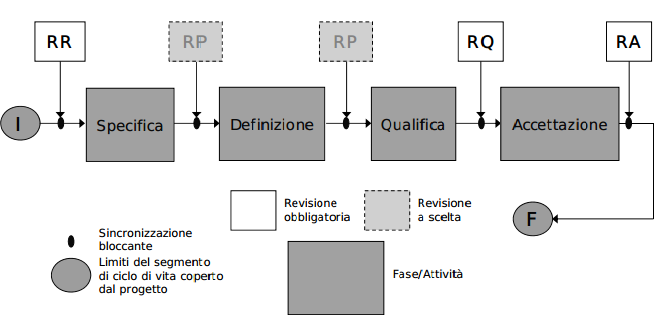
\includegraphics[width=0.75\columnwidth]{img1} % Example image
\end{center}

Il \textbf{modello incrementale} non è iterativo, perchè l'iterazione \textit{distrugge} per sostituzione e quindi è potenzialmente pericolosa. La posso avere solo in situazioni di emergenza. Un ciclo incrementale può essere visto come un "\textit{for}". Ogni passaggio di questo ciclo aggiunge cose, mi avvicino alla soluzione per approssimazioni non distruttive, quindi additive. Posso anche non incrementare ma l'importante è che il numero di iterazioni sia noto. Dentro una chiamata di RP posso portare più di un incremento. Questo è il modello maggiormente desiderato dai proponenti.

\begin{center}
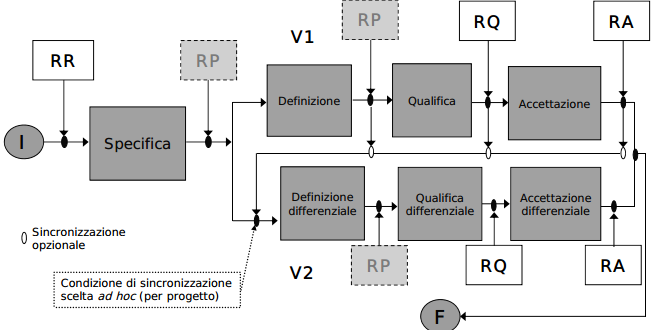
\includegraphics[width=0.75\columnwidth]{img2} % Example image
\end{center}

Posso fare un modello in stile \textit{Chrome} ("un numero grande di versioni è bello"), \textbf{modello evolutivo}. E' un modello che approssima la soluzione finale ammettendo tante iterazioni, obortendo le versioni intermedie. Per poter attuare un modello evolutivo ho bisogno di tanta energia. E' una tecnica molto interessante ma con un enorme costo.

\begin{center}
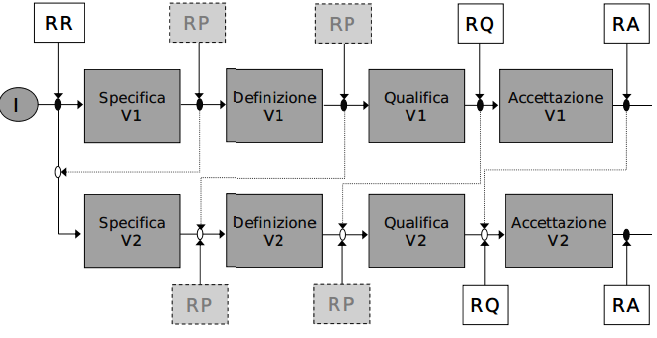
\includegraphics[width=0.75\columnwidth]{img3} % Example image
\end{center}

Gli utenti non portano innovazione ma vengono presi dall'onda dell'innovazione. Nel nostro progetto non è una scelta molto agevole.\\
Il \textbf{modello agile} non è facilmente rappresentabile. Si ragiona sulle cose da fare (\textbf{backlog}). Fra le cose da fare in un modello agile le persone prendono liberamente quello che faranno (ciascuno pesca un post-it a seconda del proprio estro). In un modello agile l'essenziale è che per ogni cosa fatta l'effetto sia visibile (\textbf{incremental build}). Ogni aggiunta rende il prodotto sempre più vicino alle aspettative, anche se non ha un ordine particolarmente ovvio. L'unico ordine è che ci siano tante cose che posso vedere e che rappresentano ciò che il prodotto sar� . E' un modello molto interessante ma difficile da gestire.

\begin{center}
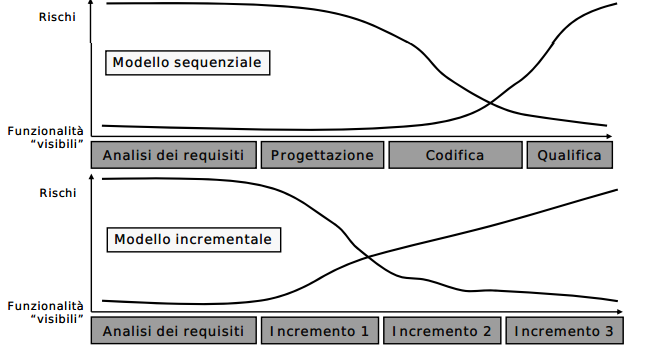
\includegraphics[width=0.75\columnwidth]{img4} % Example image
\end{center}

\textbf{Avvertenze}. Quando si è in progettazione bisogna avere la maturit�  di capire che essa deve condurre per mano lo sviluppo, deve essere la soluzione, e dev'essere verificabile in modo più o meno automatizzato. Non tutti i problemi hanno una (buona) soluzione. Bisogna fissare con la massima chiarezza:

\begin{itemize}

	\item \textbf{Obiettivi};
	\item \textbf{Vincoli};
	\item \textbf{Alternative};
	\item \textbf{Rappresentazione del problema e delle sue soluzioni}.

\end{itemize}

La prima cosa da fare è \textbf{decomporre} in modo modulare e senza dipendenze. Una buona decomposizione identifica componenti tra loro indipendenti. Le cose che decido localmente non devono avere un impatto pesante sul globale. La seconda cosa che voglio fare è esporre all'esterno solo ciò che è necessario sapere (\textbf{incapsulamento}). Voglio una forte coesione e un basso accoppiamento.\\
Si dice che l'\textbf{astrazione} sia una buona tecnica progettuale. Non importa la forma esatta che ha una cosa ma che abbia informazioni e funzionalit�  utili, non voglio sapere tutto, ma le cose importanti in un determinato contesto. Devo poter guardare alle cose che faccio con l'astrazione giusta, altrimenti se tutto è piatto sono rovinato. Quando faccio astrazione devo avere una buona percezione che l'astrazione che sto facendo sia sufficiente a caratterizzare l'entit�  desiderata. Capisco di ciò che ho bisogno, il resto è accessorio. L'astrazione che sto presentando deve essere \textbf{completa}, avere tutto ciò di cui ho bisogno. Completa per i miei scopi, niente di più. L'\textbf{atomicit� } è un altro criterio molto importante. L'utilit�  dell'astrazione non migliora se divido ulteriormente, perchè scomporre più del dovuto ha un costo.\\
\textbf{Concorrenza}, è molto importante garantire al sistema una concorrenza, ma va ben gestita e se la uso in modo inconsapevole faccio solo danni. \textbf{Distribuzione}, se e come i componenti sono disseminati su più nodi di elaborazione e come comunicano tra di loro.

\end{document}